\subsection{Assets}

\subsubsection{assets}

    Enthält Funktionalität zum asynchronen laden von Assets.

    \begin{figure}[htbp]
        \centering
        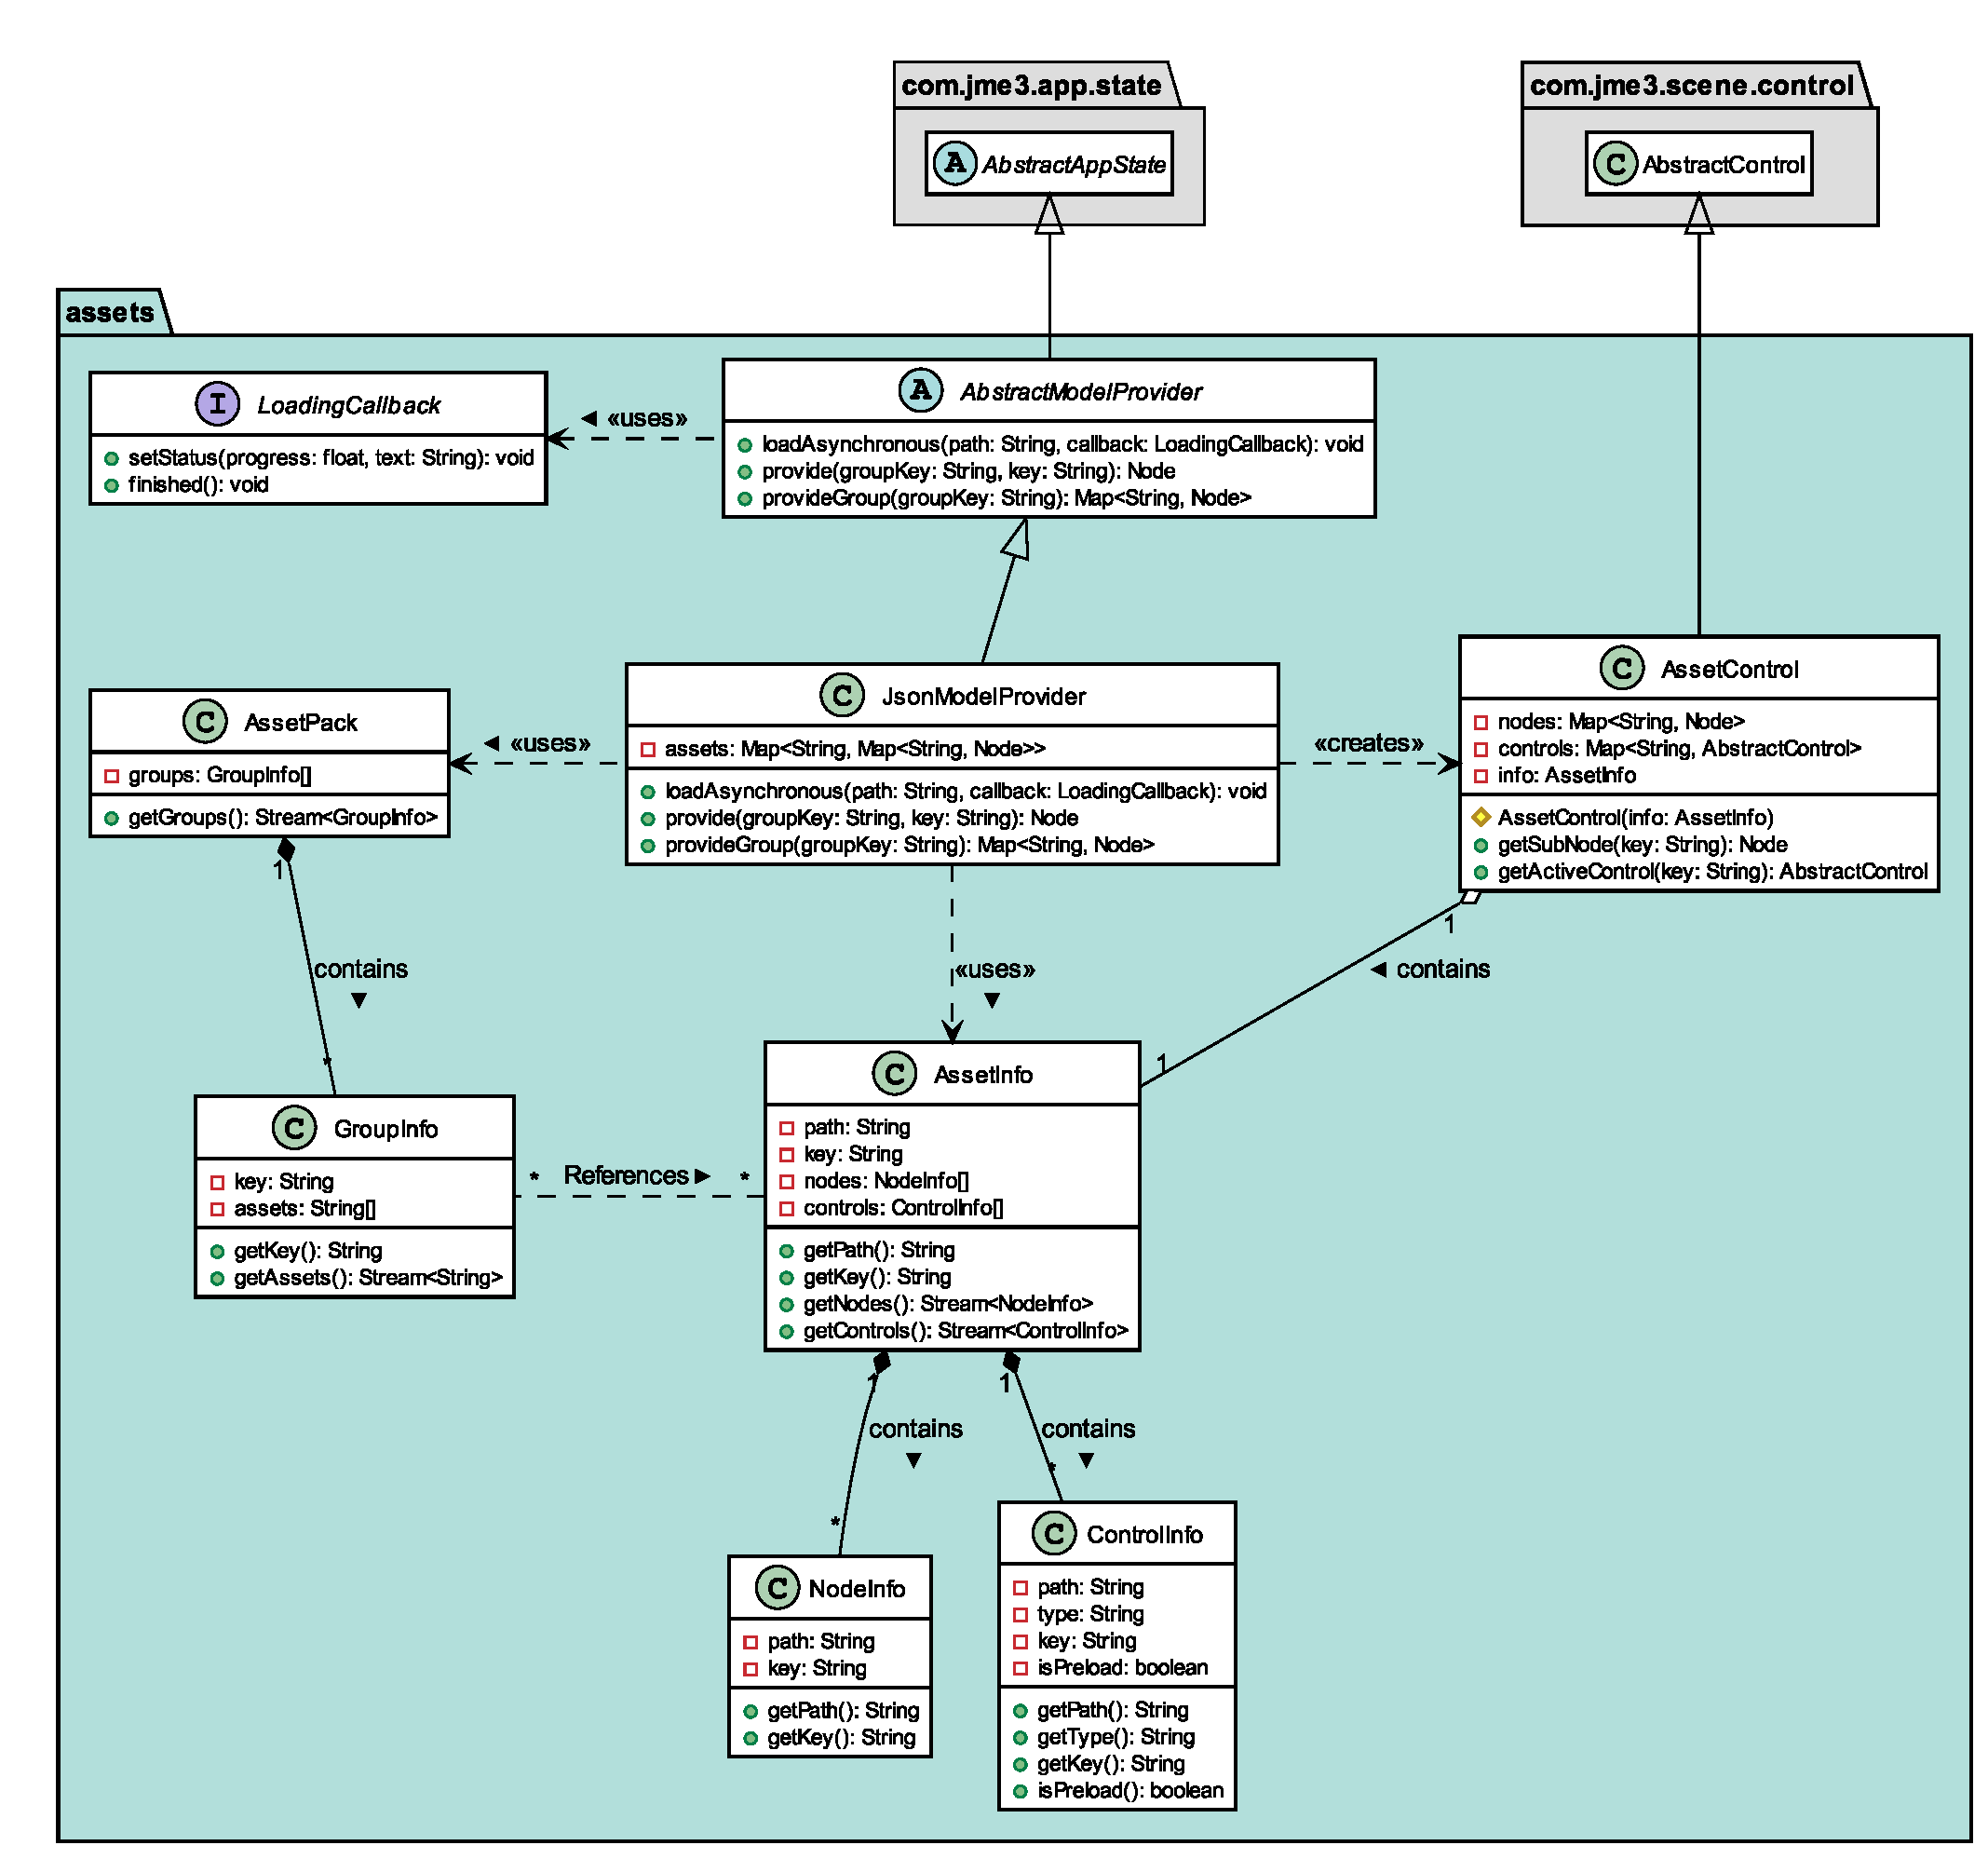
\includegraphics[width=\linewidth]{Assets/assets.eps}
        \caption{assets Klassen-Diagram}
    \end{figure}

    \pagebreak
    \paragraph{\underline{AbstractModelProvider}} \mbox{}\\
    \\
        Ein Appstate, welcher funktionalität zum laden von Assets definiert.\par

        \textbf{Methoden}
        \begin{itemize}
            \item \textit{+ loadAsynchronous(String path, LoadingCallback callback)}
                \begin{leftbar}[0.9\linewidth]
                    Lädt das \textit{AssetPack} am gegebenen Pfad in einem neuen Thread.\\
                    \textbf{@param path} Der Pfad zum \textit{AssetPack}, welches geladen werden soll.\\
                    \textbf{@param callback} Das \textit{LoadingCallback}, welches verwendet wird um dem Ladebildschirm den Status mitzuteilen.
                \end{leftbar}
            \item \textit{+ provide(String groupKey, String key): Node}
                \begin{leftbar}[0.9\linewidth]
                    Gibt ein Asset zurück.\\
                    \textbf{@param groupKey} Der Name der Gruppe zu der das Asset gehört.\\
                    \textbf{@param key} Der Name des Assets.
                \end{leftbar}
            \item \textit{+ provideGroup(String groupKey): Map<String, Node>}
                \begin{leftbar}[0.9\linewidth]
                    Gibt eine Gruppe von Assets zurück.\\
                    \textbf{@param groupKey} Der Name der Gruppe.
                \end{leftbar}
        \end{itemize}

    \paragraph{\underline{JsonModelProvider}} \mbox{}\\
    \\
        Ein \textit{AbstractModelProvider}, welcher \textit{AssetPack}s aus .json Dateien Lädt.\par

        \textbf{Attribute}
        \begin{itemize}
            \item \textit{- Map<String, Map<String, Node>> assets}
                \begin{leftbar}[0.9\linewidth]
                   Enthält alle Gruppen von Assets mit ihren Assets.
                \end{leftbar}
        \end{itemize}
        \textbf{Methoden}
        \begin{itemize}
            \item \textit{+ loadAsynchronous(String path, LoadingCallback callback)}
                \begin{leftbar}[0.9\linewidth]
                   Siehe \textit{AbstractModelProvider.loadAsynchronous()}.
                \end{leftbar}
            \item \textit{+ provide(String groupKey, String key): Node}
                \begin{leftbar}[0.9\linewidth]
                    Siehe \textit{AbstractModelProvider.provide()}.
                \end{leftbar}
            \item \textit{+ provideGroup(String groupKey): Map<String, Node>}
                \begin{leftbar}[0.9\linewidth]
                    Siehe \textit{AbstractModelProvider.provideGroup()}.
                \end{leftbar}
        \end{itemize}

    \paragraph{\underline{LoadingCallback}} \mbox{}\\
    \\
        Definiert die Schnittstelle, welche vom \textit{AbstractModelProvider} verwendet wird, um dem Ladebildschirm den Status mitzuteilen.\par

        \textbf{Methoden}
        \begin{itemize}
            \item \textit{+ setStatus(float progress, String text): void}
                \begin{leftbar}[0.9\linewidth]
                   Setzt den Status im Ladebildschirm.\\
                   \textbf{@param progress} der Fortschritt beim Laden.\\
                   \textbf{@param text} der Text der auf dem Ladebildschirm angezeigt werden soll.
                \end{leftbar}
            \item \textit{+ finished(): void}
                \begin{leftbar}[0.9\linewidth]
                    Wird aufgerufen wenn der Ladevorgang abgeschlossen wurde.
                \end{leftbar}
        \end{itemize}

    \paragraph{\underline{AssetControl}} \mbox{}\\
    \\
        Ein AbstractControl, welches Daten über das Asset, die während dem Spiel wichtig sind, speichert.\par
    
        \textbf{Attribute}
        \begin{itemize}
            \item \textit{- Map<String, Node> nodes}
                \begin{leftbar}[0.9\linewidth]
                    Enthält alle vom AssetInfo definierten Nodes mit ihrem Namen.
                \end{leftbar}
            \item \textit{- Map<String, AbstractControl> nodes}
                \begin{leftbar}[0.9\linewidth]
                    Enthält alle vom AssetInfo definierten AbstractControls mit ihrem Namen.
                \end{leftbar}
            \item \textit{- AssetInfo info}
                \begin{leftbar}[0.9\linewidth]
                    Die \textit{AssetInfo} für dieses Asset.
                \end{leftbar}
        \end{itemize}
        \textbf{Methoden}
        \begin{itemize}
            \item \textit{\# AssetControl(AssetInfo info)}
                \begin{leftbar}[0.9\linewidth]
                   Erstellt ein neues \textit{AssetControl} auf basis der gegebenen \textit{AssetInfo}.\\
                   \textbf{@param info} die \textit{AssetInfo}.
                \end{leftbar}
            \item \textit{+ getSubNode(String key): Node}
                \begin{leftbar}[0.9\linewidth]
                   Gibt die Node mit dem gegebenen Namen aus diesem Asset zurück.\\
                   \textbf{@param key} der Name der Node.
                \end{leftbar}
            \item \textit{+ getActiveControl(String key): AbstractControl}
                \begin{leftbar}[0.9\linewidth]
                   Gibt, das auf einer in dieser Node aktiven, AbstractControl mit dem gegebenen key zurück.\\
                   \textbf{@param key} der Name des AbstractControls.
                \end{leftbar}
        \end{itemize}

    \paragraph{\underline{AssetPack}} \mbox{}\\
    \\
        Datenstruktur, welche Informationen über eine Kollektion von Assets hält.\par

        \textbf{Attribute}
        \begin{itemize}
            \item \textit{- GroupInfo[] groups}
                \begin{leftbar}[0.9\linewidth]
                    Alle Gruppen von Assets in diesem \textit{AssetPack}.
                \end{leftbar}
        \end{itemize}
        \textbf{Methoden}
        \begin{itemize}
            \item \textit{+ getGroups(): Stream<GroupInfo>}
                \begin{leftbar}[0.9\linewidth]
                   \textbf{@return} alle \textit{GroupInfo}s als Stream.
                \end{leftbar}
        \end{itemize}

    \paragraph{\underline{GroupInfo}} \mbox{}\\
    \\
        Datenstruktur, welche Informationen über eine Gruppe von Assets hält.\par

        \textbf{Attribute}
        \begin{itemize}
            \item \textit{- String[] assets}
                \begin{leftbar}[0.9\linewidth]
                    Die Pfade zu allen Assets in dieser \textit{GroupInfo}.
                \end{leftbar}
            \item \textit{- String key}
                \begin{leftbar}[0.9\linewidth]
                    Der Name dieser \textit{GroupInfo}.
                \end{leftbar}
        \end{itemize}
        \textbf{Methoden}
        \begin{itemize}
            \item \textit{+ getKey(): String}
                \begin{leftbar}[0.9\linewidth]
                    \textbf{@return} Den Namen dieser \textit{GroupInfo}.
                \end{leftbar}
            \item \textit{+ getAssets(): Stream<String>}
                \begin{leftbar}[0.9\linewidth]
                    \textbf{@return} Die Pfade zu allen Assets.
                \end{leftbar}
        \end{itemize}

    \paragraph{\underline{AssetInfo}} \mbox{}\\
    \\
        Datenstruktur, welche Informationen ein Asset hält.\par

        \textbf{Attribute}
        \begin{itemize}
            \item \textit{- String path}
                \begin{leftbar}[0.9\linewidth]
                    Der Pfad zum .j3o Asset.
                \end{leftbar}
            \item \textit{- String key}
                \begin{leftbar}[0.9\linewidth]
                    Der Name dieser \textit{AssetInfo}.
                \end{leftbar}
            
            \pagebreak
            \item \textit{- NodeInfo[] nodes}
                \begin{leftbar}[0.9\linewidth]
                    Informationen über alle Nodes, welche während des Spiels erreichbar sein müssen.
                \end{leftbar}
            \item \textit{- ControlInfo[] controls}
                \begin{leftbar}[0.9\linewidth]
                    Informationen über alle AbstractControls, welche während des Spiels erreichbar sein müssen.
                \end{leftbar}
        \end{itemize}
        \textbf{Methoden}
        \begin{itemize}
            \item \textit{+ getPath(): String}
                \begin{leftbar}[0.9\linewidth]
                    \textbf{@return} Den Pfad zum .j3o Asset.
                \end{leftbar}
            \item \textit{+ getKey(): String}
                \begin{leftbar}[0.9\linewidth]
                    \textbf{@return} Den Namen dieser \textit{AssetInfo}.
                \end{leftbar}
            \item \textit{+ getNodes(): Stream<NodeInfo>}
                \begin{leftbar}[0.9\linewidth]
                    \textbf{@return} Alle \textit{NodeInfo}s von dieser \textit{AssetInfo}.
                \end{leftbar}
            \item \textit{+ getControls(): Stream<ControlInfo>}
                \begin{leftbar}[0.9\linewidth]
                    \textbf{@return} Alle \textit{ControlInfo}s von dieser \textit{AssetInfo}.
                \end{leftbar}
        \end{itemize}
        
    \paragraph{\underline{NodeInfo}} \mbox{}\\
    \\
        Datenstruktur, welche Informationen über eine Node innerhalb eines Assets hält.\par

        \textbf{Attribute}
        \begin{itemize}
            \item \textit{- String path}
                \begin{leftbar}[0.9\linewidth]
                    Der Pfad der Node.
                \end{leftbar}
            \item \textit{- String key}
                \begin{leftbar}[0.9\linewidth]
                    Der Name der Node.
                \end{leftbar}
        \end{itemize}
        \textbf{Methoden}
        \begin{itemize}
            \item \textit{+ getKey(): String}
                \begin{leftbar}[0.9\linewidth]
                    \textbf{@return} Den Namen dieser \textit{NodeInfo}.
                \end{leftbar}
            \item \textit{+ getPath(): String}
                \begin{leftbar}[0.9\linewidth]
                    \textbf{@return} Den Pfad zur Node.
                \end{leftbar}
        \end{itemize}

    \pagebreak
    \paragraph{\underline{ControlInfo}} \mbox{}\\
    \\
        Datenstruktur, welche Informationen über ein AbstractControl innerhalb eines Assets hält.\par

        \textbf{Attribute}
        \begin{itemize}
            \item \textit{- String path}
                \begin{leftbar}[0.9\linewidth]
                    Der Pfad der Node mit dem AbstractControl.
                \end{leftbar}
            \item \textit{- String type}
                \begin{leftbar}[0.9\linewidth]
                    Der volle Name des Java-Typs des AbstractControls.
                \end{leftbar}
            \item \textit{- String key}
                \begin{leftbar}[0.9\linewidth]
                    Der Name des AbstractControl.
                \end{leftbar}
            \item \textit{- boolean isPreload}
                \begin{leftbar}[0.9\linewidth]
                    Ob das AbstractControl manuell erstellt werden muss, oder bereits existiert.
                \end{leftbar}
        \end{itemize}
        \textbf{Methoden}
        \begin{itemize}
            \item \textit{+ getKey(): String}
                \begin{leftbar}[0.9\linewidth]
                    \textbf{@return} Den Namen dieser \textit{ControlInfo}.
                \end{leftbar}
            \item \textit{+ getType(): String}
                \begin{leftbar}[0.9\linewidth]
                    \textbf{@return} Den vollen Namen des Java-Typs des AbstractControls.
                \end{leftbar}
            \item \textit{+ getPath(): String}
                \begin{leftbar}[0.9\linewidth]
                    \textbf{@return} Den Pfad zur Node mit dem AbstractControl.
                \end{leftbar}
            \item \textit{+ isPreload(): boolean}
                \begin{leftbar}[0.9\linewidth]
                    \textbf{@return} Ob das AbstractControl manuell erstellt werden muss, oder bereits existiert.
                \end{leftbar}
        \end{itemize}

\pagebreak